\documentclass[border = .2cm]{standalone}
\usepackage{tikz}
\usepackage{amsmath}

\pgfdeclarelayer{bg}
\pgfsetlayers{bg,main}

\tikzstyle{vx}=[fill=gray!30, draw=black, shape=circle, minimum size=5pt, inner sep=2pt]
\tikzstyle{wire}=[-, thick]

\begin{document}
  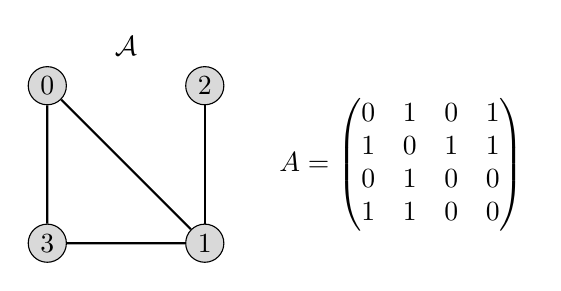
\begin{tikzpicture}
    \node [vx] (a0) at (-1, 1) {0};
    \node [vx] (a3) at (-1, -1) {3};
    \node [vx] (a2) at (1, 1) {2};
    \node [vx] (a1) at (1, -1) {1};
    \node at (0, 1.5) {$\mathcal{A}$};

    \node at (3.5, 0) {
      $A=\begin{pmatrix}
        0 & 1 & 0 & 1\\
        1 & 0 & 1 & 1\\
        0 & 1 & 0 & 0\\
        1 & 1 & 0 & 0
      \end{pmatrix}$
    };

    \begin{pgfonlayer}{bg}
        \draw [wire] (a3) -- (a0) -- (a1) -- (a3);
        \draw [wire] (a1) -- (a2);
    \end{pgfonlayer}
  \end{tikzpicture}
\end{document} 
